\begin{figure}[!h]
\centering
\resizebox{\textwidth}{!}{%
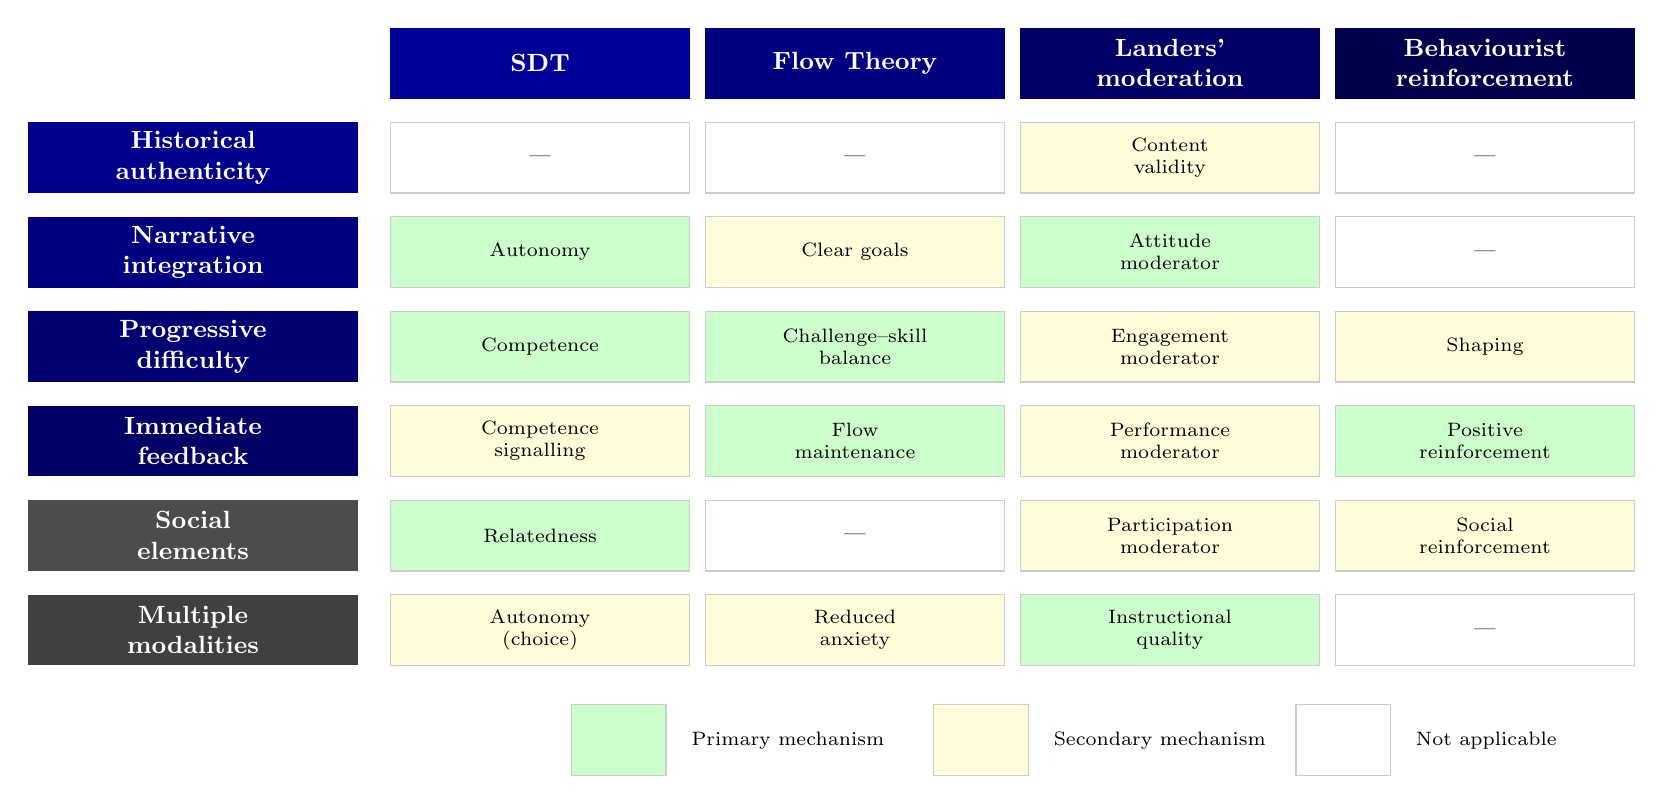
\begin{tikzpicture}[
  hdr/.style={font=\small\bfseries, text=white, minimum height=0.9cm,
    minimum width=3.8cm, align=center},
  rhdr/.style={font=\small\bfseries, text=white, minimum height=0.9cm,
    minimum width=4.2cm, align=center, anchor=east},
  cell/.style={rectangle, draw=gray!40, minimum height=0.9cm,
    minimum width=3.8cm, align=center, font=\scriptsize},
  prim/.style={cell, fill=green!20},
  sec/.style={cell, fill=yellow!15},
  none/.style={cell, fill=white},
]

% Column headers
\node[hdr, fill=blue!60!black] at (0, 0) {SDT};
\node[hdr, fill=blue!50!black] at (4.0, 0) {Flow Theory};
\node[hdr, fill=blue!40!black] at (8.0, 0) {Landers'\\moderation};
\node[hdr, fill=blue!30!black] at (12.0, 0) {Behaviourist\\reinforcement};

% Row 1: Historical authenticity
\node[rhdr, fill=blue!55!black] at (-2.3, -1.2) {Historical\\authenticity};
\node[none] at (0, -1.2) {---};
\node[none] at (4.0, -1.2) {---};
\node[sec] at (8.0, -1.2) {Content\\validity};
\node[none] at (12.0, -1.2) {---};

% Row 2: Narrative integration
\node[rhdr, fill=blue!50!black] at (-2.3, -2.4) {Narrative\\integration};
\node[prim] at (0, -2.4) {Autonomy};
\node[sec] at (4.0, -2.4) {Clear goals};
\node[prim] at (8.0, -2.4) {Attitude\\moderator};
\node[none] at (12.0, -2.4) {---};

% Row 3: Progressive difficulty
\node[rhdr, fill=blue!45!black] at (-2.3, -3.6) {Progressive\\difficulty};
\node[prim] at (0, -3.6) {Competence};
\node[prim] at (4.0, -3.6) {Challenge--skill\\balance};
\node[sec] at (8.0, -3.6) {Engagement\\moderator};
\node[sec] at (12.0, -3.6) {Shaping};

% Row 4: Immediate feedback
\node[rhdr, fill=blue!40!black] at (-2.3, -4.8) {Immediate\\feedback};
\node[sec] at (0, -4.8) {Competence\\signalling};
\node[prim] at (4.0, -4.8) {Flow\\maintenance};
\node[sec] at (8.0, -4.8) {Performance\\moderator};
\node[prim] at (12.0, -4.8) {Positive\\reinforcement};

% Row 5: Social elements
\node[rhdr, fill=gray!60!black] at (-2.3, -6.0) {Social\\elements};
\node[prim] at (0, -6.0) {Relatedness};
\node[none] at (4.0, -6.0) {---};
\node[sec] at (8.0, -6.0) {Participation\\moderator};
\node[sec] at (12.0, -6.0) {Social\\reinforcement};

% Row 6: Multiple modalities
\node[rhdr, fill=gray!50!black] at (-2.3, -7.2) {Multiple\\modalities};
\node[sec] at (0, -7.2) {Autonomy\\(choice)};
\node[sec] at (4.0, -7.2) {Reduced\\anxiety};
\node[prim] at (8.0, -7.2) {Instructional\\quality};
\node[none] at (12.0, -7.2) {---};

% Legend
\node[prim, minimum width=1.2cm] at (1.0, -8.6) {};
\node[font=\scriptsize, anchor=west] at (1.8, -8.6) {Primary mechanism};
\node[sec, minimum width=1.2cm] at (5.6, -8.6) {};
\node[font=\scriptsize, anchor=west] at (6.4, -8.6) {Secondary mechanism};
\node[none, minimum width=1.2cm] at (10.2, -8.6) {};
\node[font=\scriptsize, anchor=west] at (11.0, -8.6) {Not applicable};

\end{tikzpicture}%
}% end resizebox
\caption{Theoretical grounding of the six design principles. Historical authenticity (top row) lacks general-theory support, reflecting its status as a discipline-specific principle unique to history education gamification.}
\label{fig:principle-theoretical-grounding}
\end{figure}
